\chapter{Benchmarks}
\section{Data Overhead}
Data Overhead is besides the latency one of the most important metrics especially for a geo distributed system like a smart grid due to usally strong bandwidth limitations. Therefore it's very important to know which additional "message costs" are related to the use of our provenance system.

We performed several experiments with different provenance configurations as well experiments completely without provenance to determine how big the impact for the use of the provenance system is. We wanted also to determine which setting has more impact of the overhead and which has less to give a recommendation on a possible setup dependent on available bandwidth.
We did the benchmarks for different topologies that stands for usual patterns in real topologies. For each topology we will describe our assumptions and then evalute the results of that.

\subsection{Test Setup}
To run the equal testconfiguration on every topology, we wrote a script\footnote{available in the repository \texttt{/benchmarks/overhead/benchmark.sh}} that go through the steps as in figure \ref{fig:benchmark}.
The benchmark script runs a 120 seconds long benchmark run on each topology with all combinations of the following configurations:


\begin{itemize}
\item metrics configuration :

We executed runs with full provenance (\texttt{meterid,metricid,loc,line,class,app,ctime,stime,rtime}) and made runs with each inidvidual metric together with \texttt{ctime}, because this metric is mandatory for the correct function of the system.

\item buffer sizes : \texttt{1,5,10}
\end{itemize}


\begin{figure}[H]
	\center
	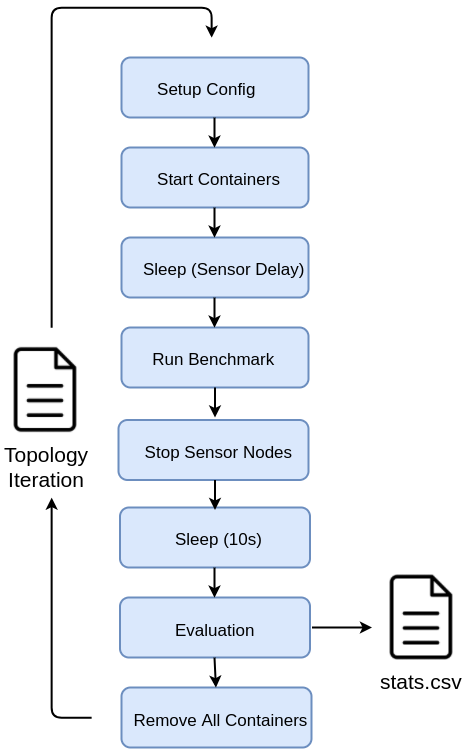
\includegraphics[width=0.5\textwidth]{figures/dataoverheadsetup.png}
	\caption{Benchmark Procedure}
	\label{fig:benchmark}
\end{figure}

The benchmark runs this combinations for each topology file that is defined inside the script. On the first step the respective metrics and buffer configrations are replaced in the compose file that contains the topology.
The the containers are started by \emph{docker-compose}. In the script is a fixed startup-delay for the sensors defined. This is needed to ensure that all containers are running at the beginning of the benchmark. On the "Run Benchmark" step, the script waits until the defined benchmark time of 120 seconds are expired. Then only the workload generator nodes are switched of. Another waiting time (10 seconds) is used to ensure that the sensor nodes are terminated and no pending messages are on the pipeline. Then the \emph{docker stats}\footnote{\url{https://docs.docker.com/engine/reference/commandline/stats/}} command is executed to get the \texttt{Net I/O} metrics for each node. In addition to the docker stats, all local storages of the pipeline nodes are queried to get the number of messages that passed through the node. The retrieved stats are stored to a csv file that is created at the beginning of the script.
After "Evaluation" all containers are stopped and removed to guarantee that no run is influenced by an preceeding run by already "used" containers.

The fields of the measurements are:

\begin{itemize}
\item TOPOLOGY - the topology file that was used for the run
\item PROV\_METRICS - provenance metrics that was inserted to the config
\item BUFFER\_CAPACITY - provenance buffer config
\item COMPONENT - component of the pipeline
\item NET\_IN - NET\_IN stat from docker stats
\item NET\_IN\_TYPE - format of the NET\_IN value (B,kB,MB) 
\item NET\_OUT - NET\_OUT stat from docker stats
\item NET\_OUT\_TYPE - format of the NET\_OUT value (B,kB,MB) 
\item MSG\_NUMBER - number of messages that passed the component
\item NORMALIZED\_MSG\_SIZE\_IN - NET\_IN divided by MSG\_NUMBER
\item NORMALIZED\_MSG\_SIZE\_OUT - NET\_OUT divided by MSG\_NUMBER
\item NORMALIZED\_MSG\_SIZE\_TYPE - format (B,kb,MB)
\item BENCHMARK\_RUNTIME - runtime in seconds for the benchmark
\end{itemize}



\subsection{Test Cases}
\paragraph*{Single-Node Topology}
The purpose of the Single-Node Topology is to get the pure overhead that is produced only for one data item without any passthrough of messages to other pipeline components.

\begin{figure}[H]
	\center
	
\includegraphics[width=0.3\textwidth]{figures/dataoverheadtopolabeled0.png}
	\caption{One-Node Topology}
	\label{fig:onetodetopology}
\end{figure}

We evaluated the proportion of the respective metrics by running each metric in a different run and divided the network output by the number of messages that was passed received by the component. Because the metric is a mandatory metric for every run, we substracted the run where only "ctime" was measured from all other runs. "ctime + base" is the run where only ctime was choosen as a metric. Using the network traffic to measure the impact of a metric shows not the real size of a single message. In this measurements are also the communication traffic (e.g. communication between node and cassandra db or traffic between node and docker). Even if the sizes are not the real message sizes, the diagram shows nevertheless the impact to the network traffic by choosing different metrics compared to the non provenance case.

\begin{figure}[H]
	\center
	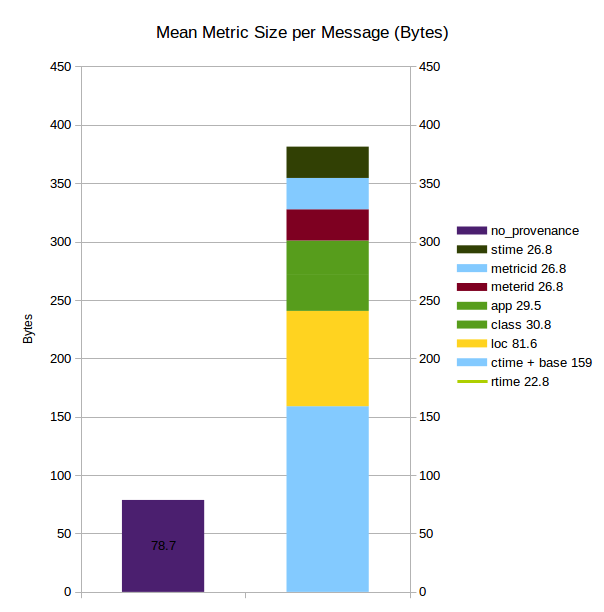
\includegraphics[width=0.7\textwidth]{figures/overheaddiagram1.png}
	\caption{Size Distribution for Metrics per Message}
	\label{fig:metricsdistribution}
\end{figure}


Do determine the message size of the measurement, we  used  "NORMALIZED\_MSG\_SIZE\_IN" stats of the endpoint for the "no\_provenance" case.

The diagramm \ref{fig:metricsdistribution} shows, that the basic metrics and the location ("loc") are the largest parts of the message. The whole traffic is approximately 5 times bigger when the provenance system is used.


\begin{figure}[H]
	\center
	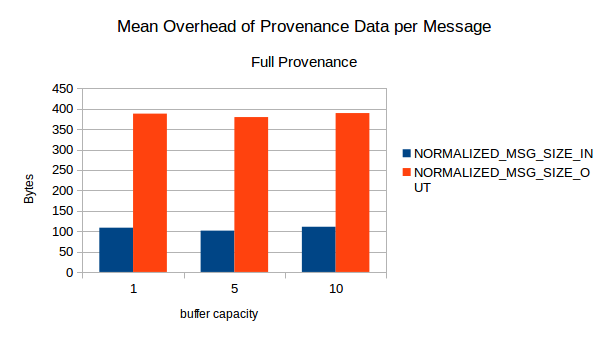
\includegraphics[width=\textwidth]{figures/overheaddiagram2.png}
	\caption{Different Buffer Sizes (Topology 0)}
	\label{fig:buffersizes}
\end{figure}

By using different buffersizes (1,5,10) no improvement can be observed on diagramm \ref{fig:buffersizes}. This option may not improve the used bandwidth due to already existing buffer mechanisms in the the used technologies for the system.


\paragraph*{Two-Node Topology}
Running the benchmark on the Two-Node topology serves to get informations if the overhead on a next node level differs from the preceeding node level. This topology consists of one sensor and two pipeline nodes (Gateway, Endpoint) which produces provenance data.

\begin{figure}[H]
	\center
	
\includegraphics[width=0.5\textwidth]{figures/dataoverheadtopolabeled1.png}
	\caption{Two-Node Topology}
	\label{fig:topo1}
\end{figure}

\begin{figure}[H]
	\center
	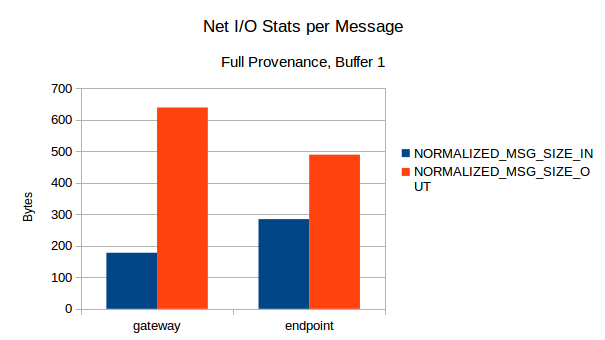
\includegraphics[width=\textwidth]{figures/overheaddiagram3.png}
	\caption{Mean Net I/O per Message (Topology 1)}
	\label{fig:topo1meanpermsg}
\end{figure}



\begin{figure}[H]
	\center
	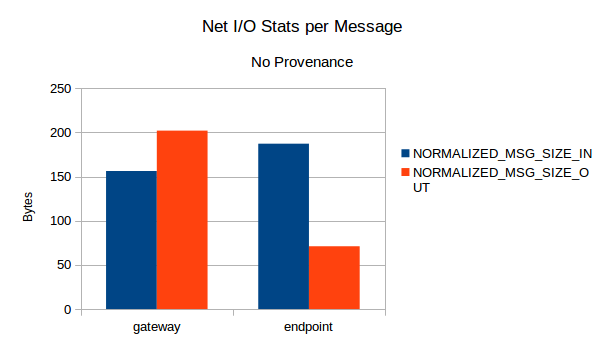
\includegraphics[width=\textwidth]{figures/overheaddiagram7.png}
	\caption{Absolute Net I/O for 7480 Messages (Topology 1)}
	\label{fig:topo1absolutenoprov}
\end{figure}

The diagram \ref{fig:topo1meanpermsg} shows, that the per message size of the gateway node is approximately 100 bytes larger than for the endpoint. That suites well to our measurement in diagramm \ref{fig:buffersizes}\footnote{The NORMALIZED\_MSG\_SIZE\_IN in \ref{fig:buffersizes} is around 100 Bytes large. This value can be interpreted as the data size of a single smart grid measurment}. The difference between the NORMALIZED\_MSG\_SIZE\_IN value of gateway and endpoint can be interpreted as the overhead if we assume that the "IN" value of the gateway stands for a measurment of sensor without provenance. The overhead in that case would be therefore round 100 bytes of data that is pushed to the next node (besides the provenance data that is also being sent to the provenance db). Here as well, it needs to be taken into account that these values are not pure message overheads but an overall impact of the whole system. For example the I/O stats also contains the Heartbeat-Messages that was send between gateway and endpoint.


\begin{figure}[H]
	\center
	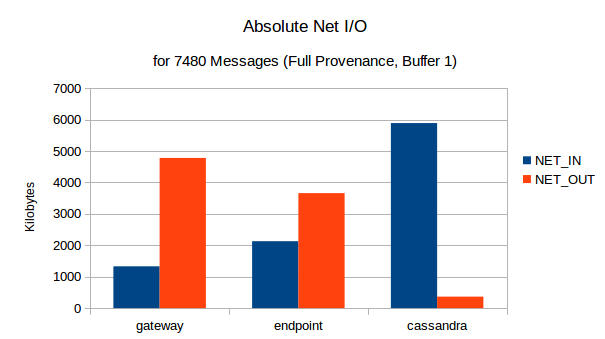
\includegraphics[width=\textwidth]{figures/overheaddiagram4.png}
	\caption{Absolute Net I/O for 7480 Messages (Topology 1)}
	\label{fig:topo1absoluteprov}
\end{figure}


\begin{figure}[H]
	\center
	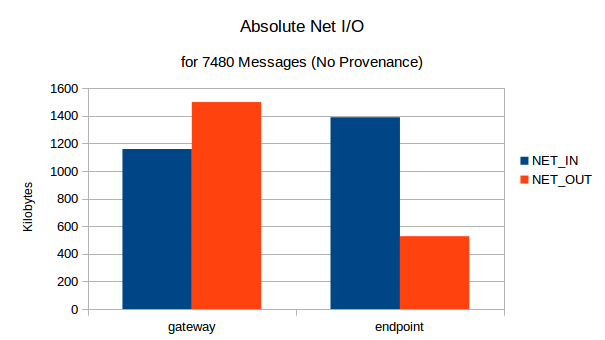
\includegraphics[width=\textwidth]{figures/overheaddiagram8.png}
	\caption{Absolute Net I/O for 7480 Messages (Topology 1)}
	\label{fig:topo1absolutewithouotprov}
\end{figure}



\paragraph*{Fork-Node Topology}
The Fork-Node topology consists of two sensor nodes which sends the measurements to two different gateways. These gateways (Gateway A,B) pushes the data to a common Gateway C. This Gateway sends the data further to antother endpoint node.

\begin{figure}[H]
	\center
	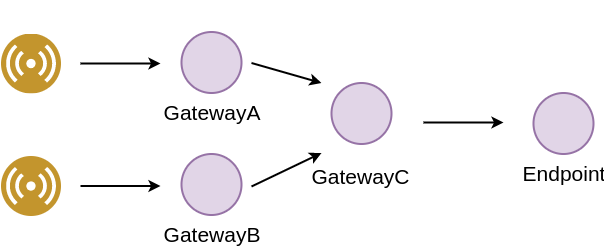
\includegraphics[width=0.7\textwidth]{figures/dataoverheadtopolabeled2.png}
	\caption{Fork-Node Topology}
	\label{fig:deployment}
\end{figure}


On this run of the benchmark we want answer the question whether the data overhead is growing on common gateways. As it can be observed in diagramm \ref{overhead5} is the \texttt{NORMALIZED\_MSG\_SIZE\_IN} approximately 100 bytes larger than for gatewayA and gatewayB. This matches our observations in the previous benchmarks.
If we compare diagram \ref{overhrad5} (Full Provenance) and  \ref{overhead6}, we can observe that the Net I/O for gatewayC grows. It's difficult to get an explanation why the mean data is bigger. One would expect that there is no difference between different gateways at least for the non-provenance case.
However, we can assume that this growth of data traffic for gatewayC is not from the provenance system itself but from the pipeline implementation.


\begin{figure}[H]
	\center
	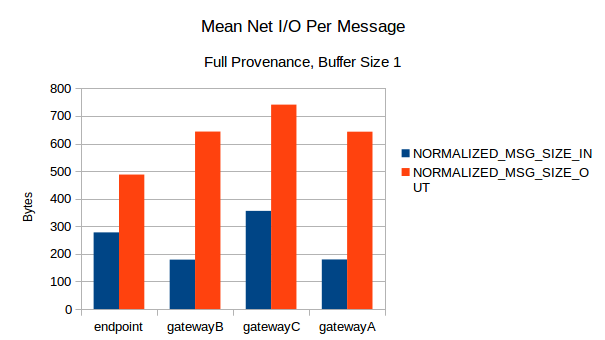
\includegraphics[width=\textwidth]{figures/overheaddiagram5.png}
	\caption{Mean Net I/O per Message (Topolgy 2)}
	\label{fig:overhrad5}
\end{figure}

\begin{figure}[H]
	\center
	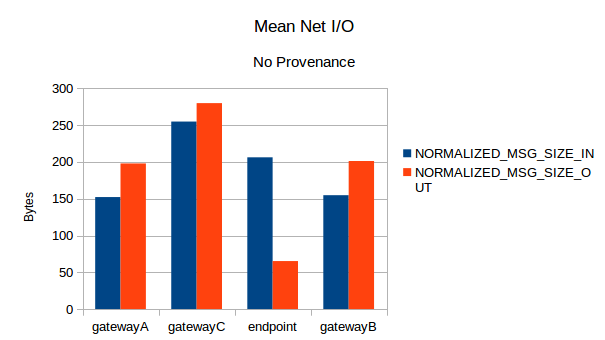
\includegraphics[width=\textwidth]{figures/overheaddiagram6.png}
	\caption{Mean Net I/O per Message (Topology 2)}
	\label{fig:overhead6}
\end{figure}


\subsection{Conclusion}
The data overhead was in our tests up to 5 times bigger than the real measurment data. This way also the case, when we used the minimal possible configuration for metrics \ref{fig:metricsdistribution} (2 times bigger).
This has to be take into account if this system ought to be used in bandwith limited environments.
Nevertheless we can assume when would have larger measurment messages, the provenance data will not be larger than in our measurements because the size of our metrics does not grow with larger measurements.
As already mentioned in the evaluation steps, the calculated mean values for the Net I/O are representing the full impact of the provenance system to the network interfaces and does not reflect the real size of messages.
